%%
%% sample document for AAMAS'18 conference
%%
%% modified from sample-sigconf.tex
%%
%% see ACM instructions acmguide.pdf
%%
%% AAMAS-specific questions? n.yorke-smith@tudelft.nl
%%

\documentclass[sigconf]{aamas}  % do not change this line!

%% your usepackages here, for example:
\usepackage{booktabs}

%% do not change the following lines
%\setcopyright{ifaamas}  % do not change this line!
%\acmDOI{doi}  % do not change this line!
%\acmISBN{}  % do not change this line!
%\acmConference[AAMAS'18]{Proc.\@ of the 17th International Conference on Autonomous Agents and Multiagent Systems (AAMAS 2018), M.~Dastani, G.~Sukthankar, E.~Andre, S.~Koenig (eds.)}{July 2018}{Stockholm, Sweden}  % do not change this line!
%\acmYear{2018}  % do not change this line!
%\copyrightyear{2018}  % do not change this line!
%\acmPrice{}  % do not change this line!

%% the rest of your preamble here
\usepackage{listings}
\usepackage{color}
\usepackage{enumitem}

\setlist[itemize]{leftmargin=*}


\lstset{frame=tb,
  language=Java,
  aboveskip=3mm,
  belowskip=3mm,
  showstringspaces=false,
  columns=flexible,
  basicstyle={\small\ttfamily},
  numbers=none,
  breaklines=true,
  breakatwhitespace=true,
  tabsize=3
}

%%%%%%%%%%%%%%%%%%%%%%%%%%%%%%%%%%%%%%%%%%%%%%%%%%%%%%%%%%%%%%%%%%%%%%%%%%%%%%%%%%%%%%%%%%%%%%%%%%%%%%%%%

\begin{document}

\title{Cryptocurrency price monitoring web application design}  % put your title here!
\subtitle{Team : 640}
%\titlenote{Produces the permission block, and copyright information}

% AAMAS: as appropriate, uncomment one subtitle line; check the CFP
%\subtitle{Extended Abstract}
%\subtitle{Industrial Applications Track}
%\subtitle{Socially Interactive Agents Track}
%\subtitle{Blue Sky Ideas Track}
%\subtitle{Robotics Track}
%\subtitle{JAAMAS Track}
%\subtitle{Doctoral Mentoring Program}

%\subtitlenote{The full version of the author's guide is available as \texttt{acmart.pdf} document}


% AAMAS: submissions are anonymous for most tracks
\author{Yuqing Cheng, Peng Tong, Xue Zhao, Yuan Gao}  % put your paper number here!

%% example of author block for camera ready version of accepted papers: don't use for anonymous submissions
%
%\author{Ben Trovato}
%\authornote{Dr.~Trovato insisted his name be first.}
%\orcid{1234-5678-9012}
%\affiliation{%
%  \institution{Institute for Clarity in Documentation}
%  \streetaddress{P.O. Box 1212}
%  \city{Dublin} 
%  \state{Ohio} 
%  \postcode{43017-6221}
%}
%\email{trovato@corporation.com}
%
%\author{G.K.M. Tobin}
%\authornote{The secretary disavows any knowledge of this author's actions.}
%\affiliation{%
%  \institution{Institute for Clarity in Documentation}
%  \streetaddress{P.O. Box 1212}
%  \city{Dublin} 
%  \state{Ohio} 
%  \postcode{43017-6221}
%}
%\email{webmaster@marysville-ohio.com}
%
%\author{Lars Th{\o}rv{\"a}ld}
%\authornote{This author is the
%  one who did all the really hard work.}
%\affiliation{%
%  \institution{The Th{\o}rv{\"a}ld Group}
%  \streetaddress{1 Th{\o}rv{\"a}ld Circle}
%  \city{Hekla} 
%  \country{Iceland}}
%\email{larst@affiliation.org}
%
%\author{Valerie B\'eranger}
%\affiliation{%
%  \institution{Inria Paris-Rocquencourt}
%  \city{Rocquencourt}
%  \country{France}
%}
%\author{Aparna Patel} 
%\affiliation{%
% \institution{Rajiv Gandhi University}
% \streetaddress{Rono-Hills}
% \city{Doimukh} 
% \state{Arunachal Pradesh}
% \country{India}}
%\author{Huifen Chan}
%\affiliation{%
%  \institution{Tsinghua University}
%  \streetaddress{30 Shuangqing Rd}
%  \city{Haidian Qu} 
%  \state{Beijing Shi}
%  \country{China}
%}
%
%\author{Charles Palmer}
%\affiliation{%
%  \institution{Palmer Research Laboratories}
%  \streetaddress{8600 Datapoint Drive}
%  \city{San Antonio}
%  \state{Texas} 
%  \postcode{78229}}
%\email{cpalmer@prl.com}
%
%\author{John Smith}
%\affiliation{\institution{The Th{\o}rv{\"a}ld Group}}
%\email{jsmith@affiliation.org}
%
%\author{Julius P.~Kumquat}
%\affiliation{\institution{The Kumquat Consortium}}
%\email{jpkumquat@consortium.net}
%
%% The example's default list of authors is too long for headers
%\renewcommand{\shortauthors}{B. Trovato et al.}


%\begin{abstract}  % put your abstract here!

%\end{abstract}


% AAMAS: the ACM CCS are not needed within AAMAS papers
%%
%% The code below should be generated by the tool at
%% http://dl.acm.org/ccs.cfm
%% Please copy and paste the code instead of the example below. 
%%
%\begin{CCSXML}
%<ccs2012>
% <concept>
%  <concept_id>10010520.10010553.10010562</concept_id>
%  <concept_desc>Computer systems organization~Embedded systems</concept_desc>
%  <concept_significance>500</concept_significance>
% </concept>
% <concept>
%  <concept_id>10010520.10010575.10010755</concept_id>
%  <concept_desc>Computer systems organization~Redundancy</concept_desc>
%  <concept_significance>300</concept_significance>
% </concept>
% <concept>
%  <concept_id>10010520.10010553.10010554</concept_id>
%  <concept_desc>Computer systems organization~Robotics</concept_desc>
%  <concept_significance>100</concept_significance>
% </concept>
% <concept>
%  <concept_id>10003033.10003083.10003095</concept_id>
%  <concept_desc>Networks~Network reliability</concept_desc>
%  <concept_significance>100</concept_significance>
% </concept>
%</ccs2012>  
%\end{CCSXML}
%
%\ccsdesc[500]{Computer systems organization~Embedded systems}
%\ccsdesc[300]{Computer systems organization~Redundancy}
%\ccsdesc{Computer systems organization~Robotics}
%\ccsdesc[100]{Networks~Network reliability}


%\keywords{Pacman; Multi-player; Minimax; Particle Filter}  % put your semicolon-separated keywords here!

\maketitle


%%%%%%%%%%%%%%%%%%%%%%%%%%%%%%%%%%%%%%%%%%%%%%%%%%%%%%%%%%%%%%%%%%%%%%%%%%%%%%%%%%%%%%%%%%%%%%%%%%%%%%%%%
%% start of main body of paper

\section{Introduction and App Description}



\section{Interact with application}
There are four main pages in our application.
\subsection{Index Page}
Index page contains three main parts: navbar, news, and coin info of three types 
of cryptocurrency.
\begin{itemize}
\item If the user is not logged in, he/she can only see the log in and sign up
dropdown on the navbar. 
\item By clicking the log in dropdown, the user can log in with google or github
account. Or he/she can log in using his/her own account on our website.
\item By clicking the sign up dropdown, the user can sign up an account on our 
website.
\item If the user is logged in, he/she can access coins info page, alert page
and notification center page via button on navbar.
\item Left part of main body in index is news part, where our application will
show the latest cryptocurrency news. By clicking the news title, we can view the
detail of that new on news websites.
\item Right part of main body in index is coin info part, where our application 
will show the real time price, change since open, and open price of three different 
coins(BTC, ETH, LTC). By clicking the coin name, we can enter the specific info 
page of that type of coin.
\begin{figure}[!htb]
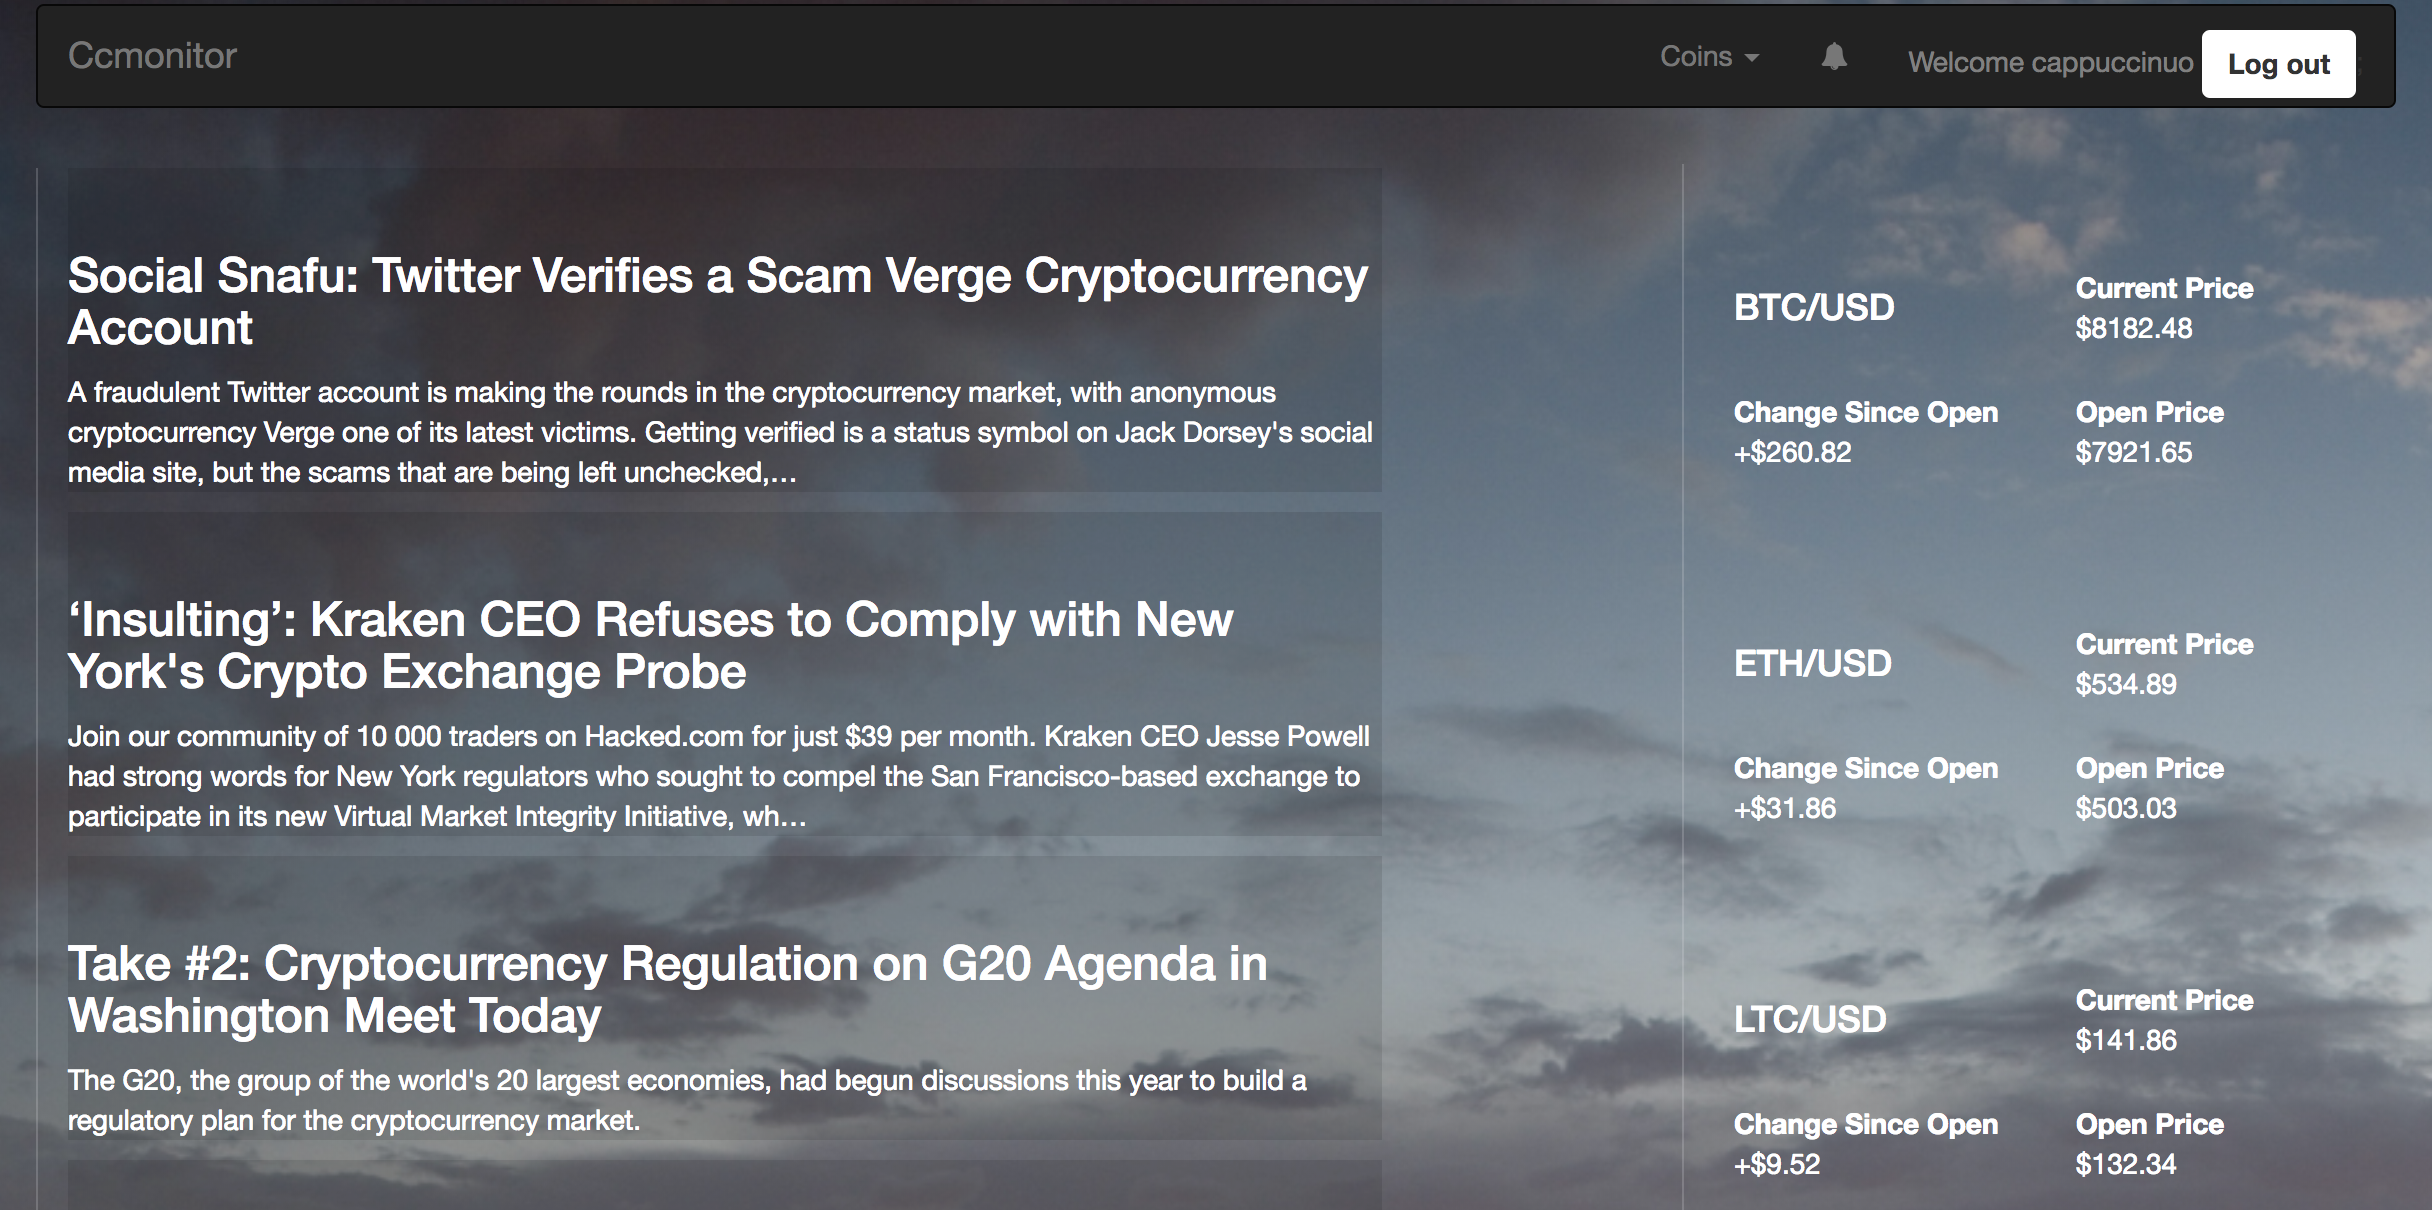
\includegraphics[height=2.0in, width=3.5in]{index.png}
\caption{\texttt{Index Page}}
\end{figure}
\end{itemize}

\subsection{Coin Info Page}
The coin page show specific info of each coin. On the top of the page, we display 
the same brief information on index of that coin. Right of that part we use a chart
to display the trend of that coin, including real time price trend, day price trend,
week price trend and month price trend. On the bottom part of the page, we display
a table that shows 30 days historical price of that coin.
\begin{figure}[!htb]
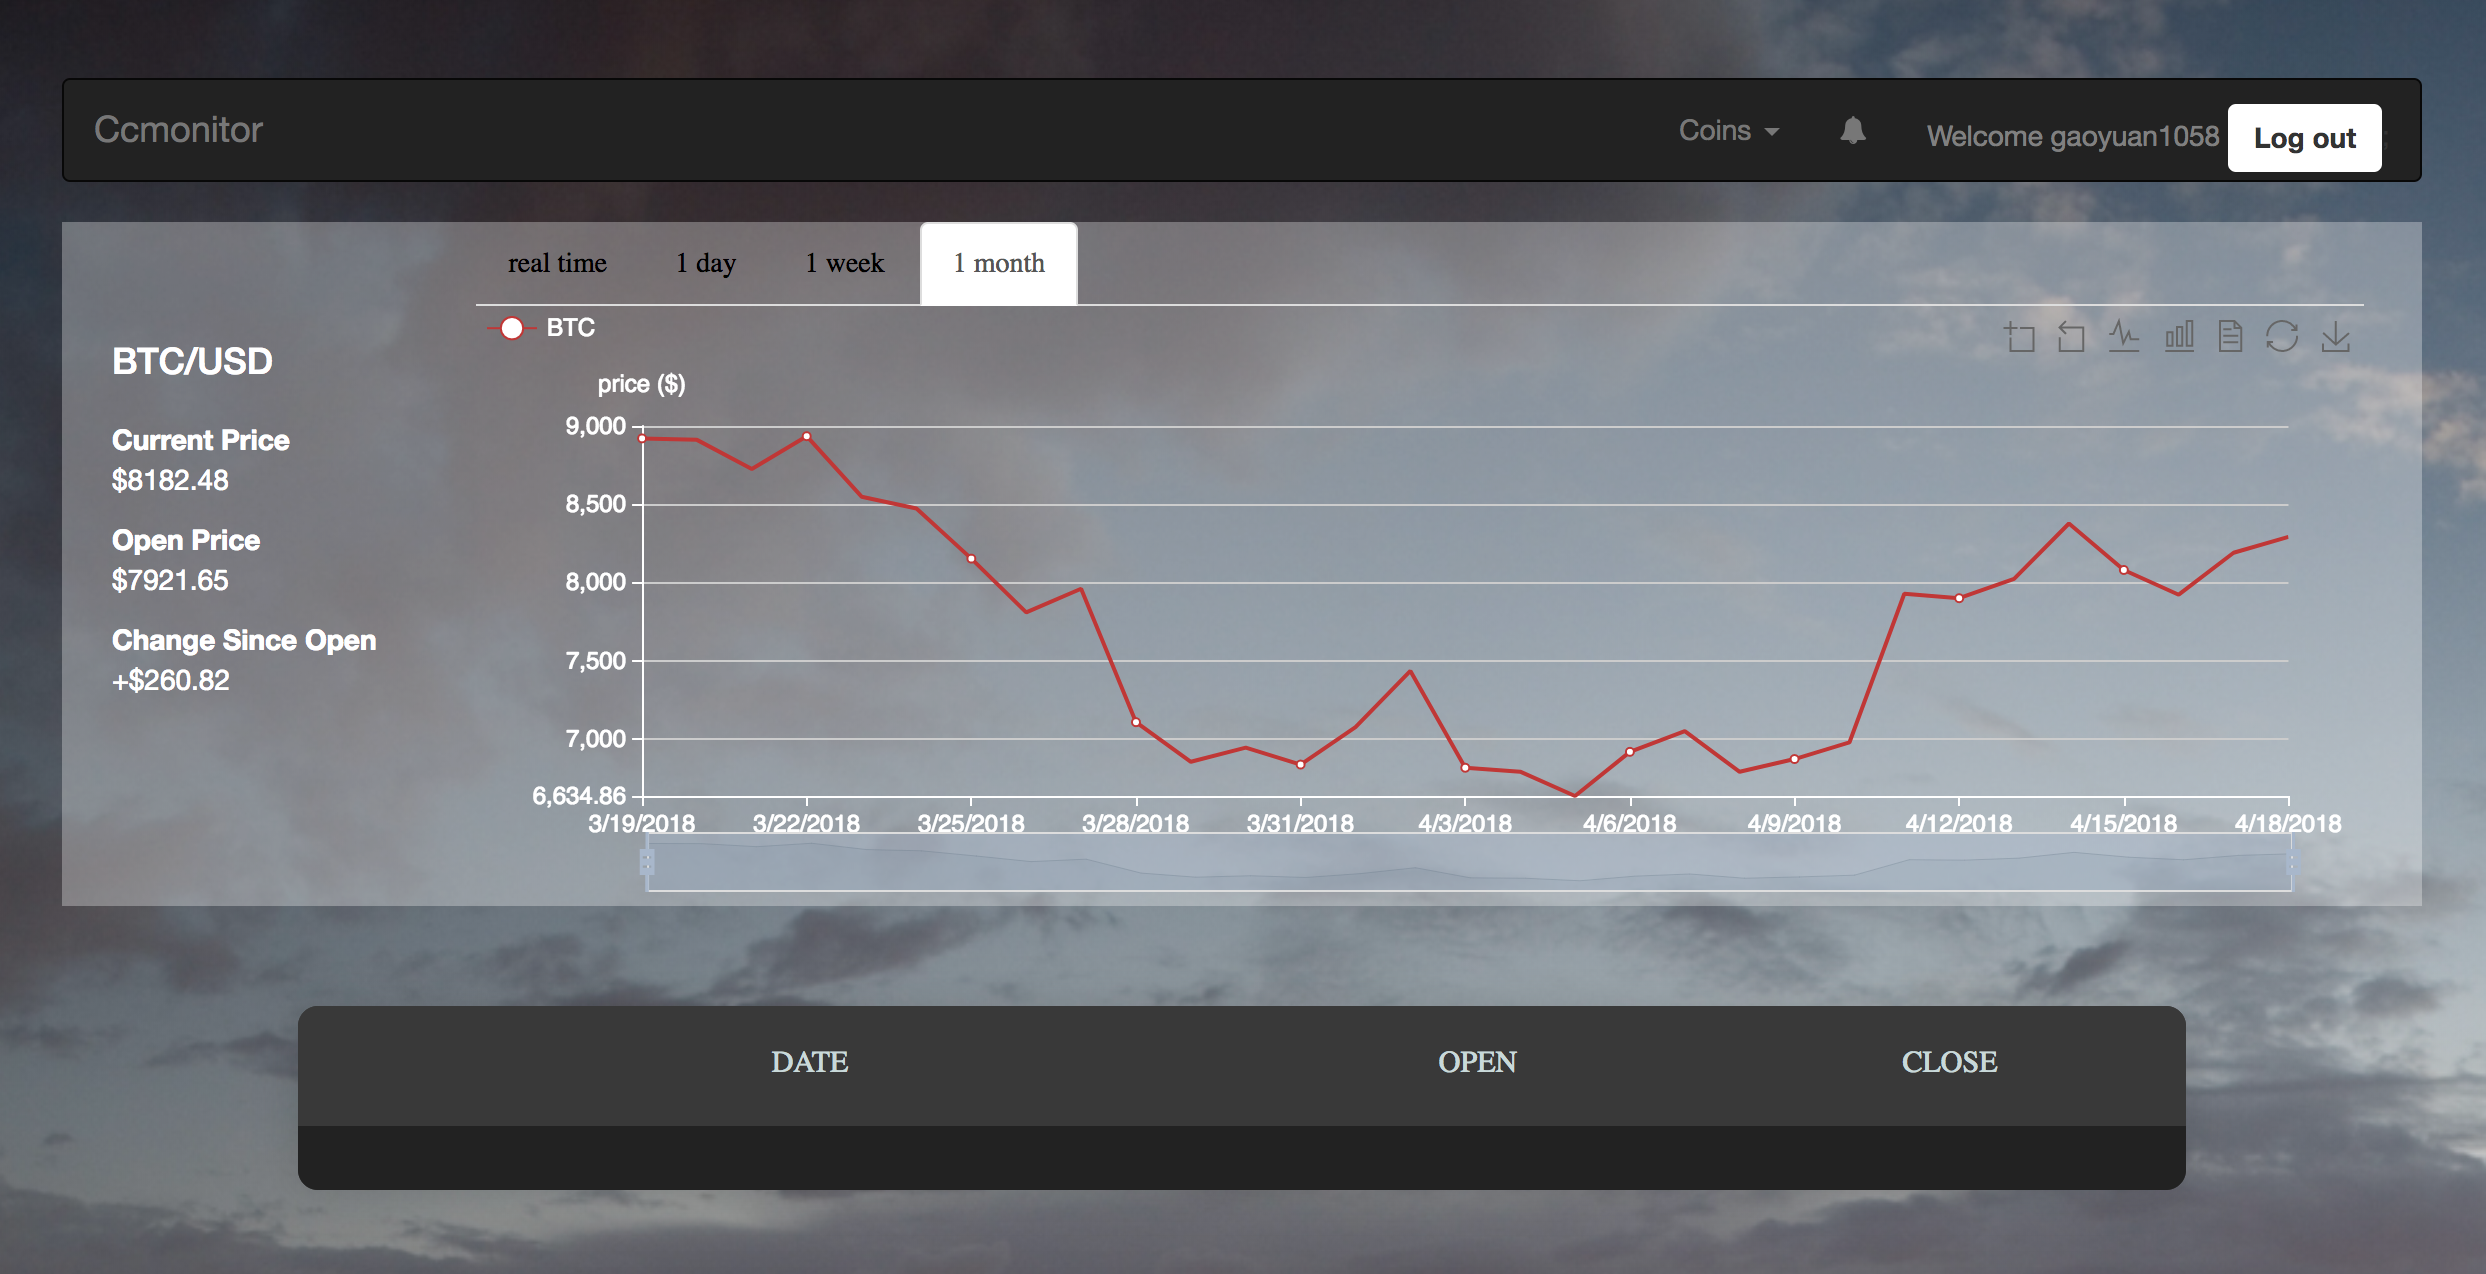
\includegraphics[height=2.0in, width=3.5in]{coinpage.png}
\caption{\texttt{BitCoin Info Page}}
\end{figure}

\subsection{Alert Page}
There are two parts of our alert page, new subscribe and my alert.

To subsribe a new alert, the user can click coins on nav bar and click subsribe. Users
can choose coin type(BTC, LTC, ETH), alert type(Ascending or Descending), as well as the 
threshold of that alert.

\begin{figure}[!htb]
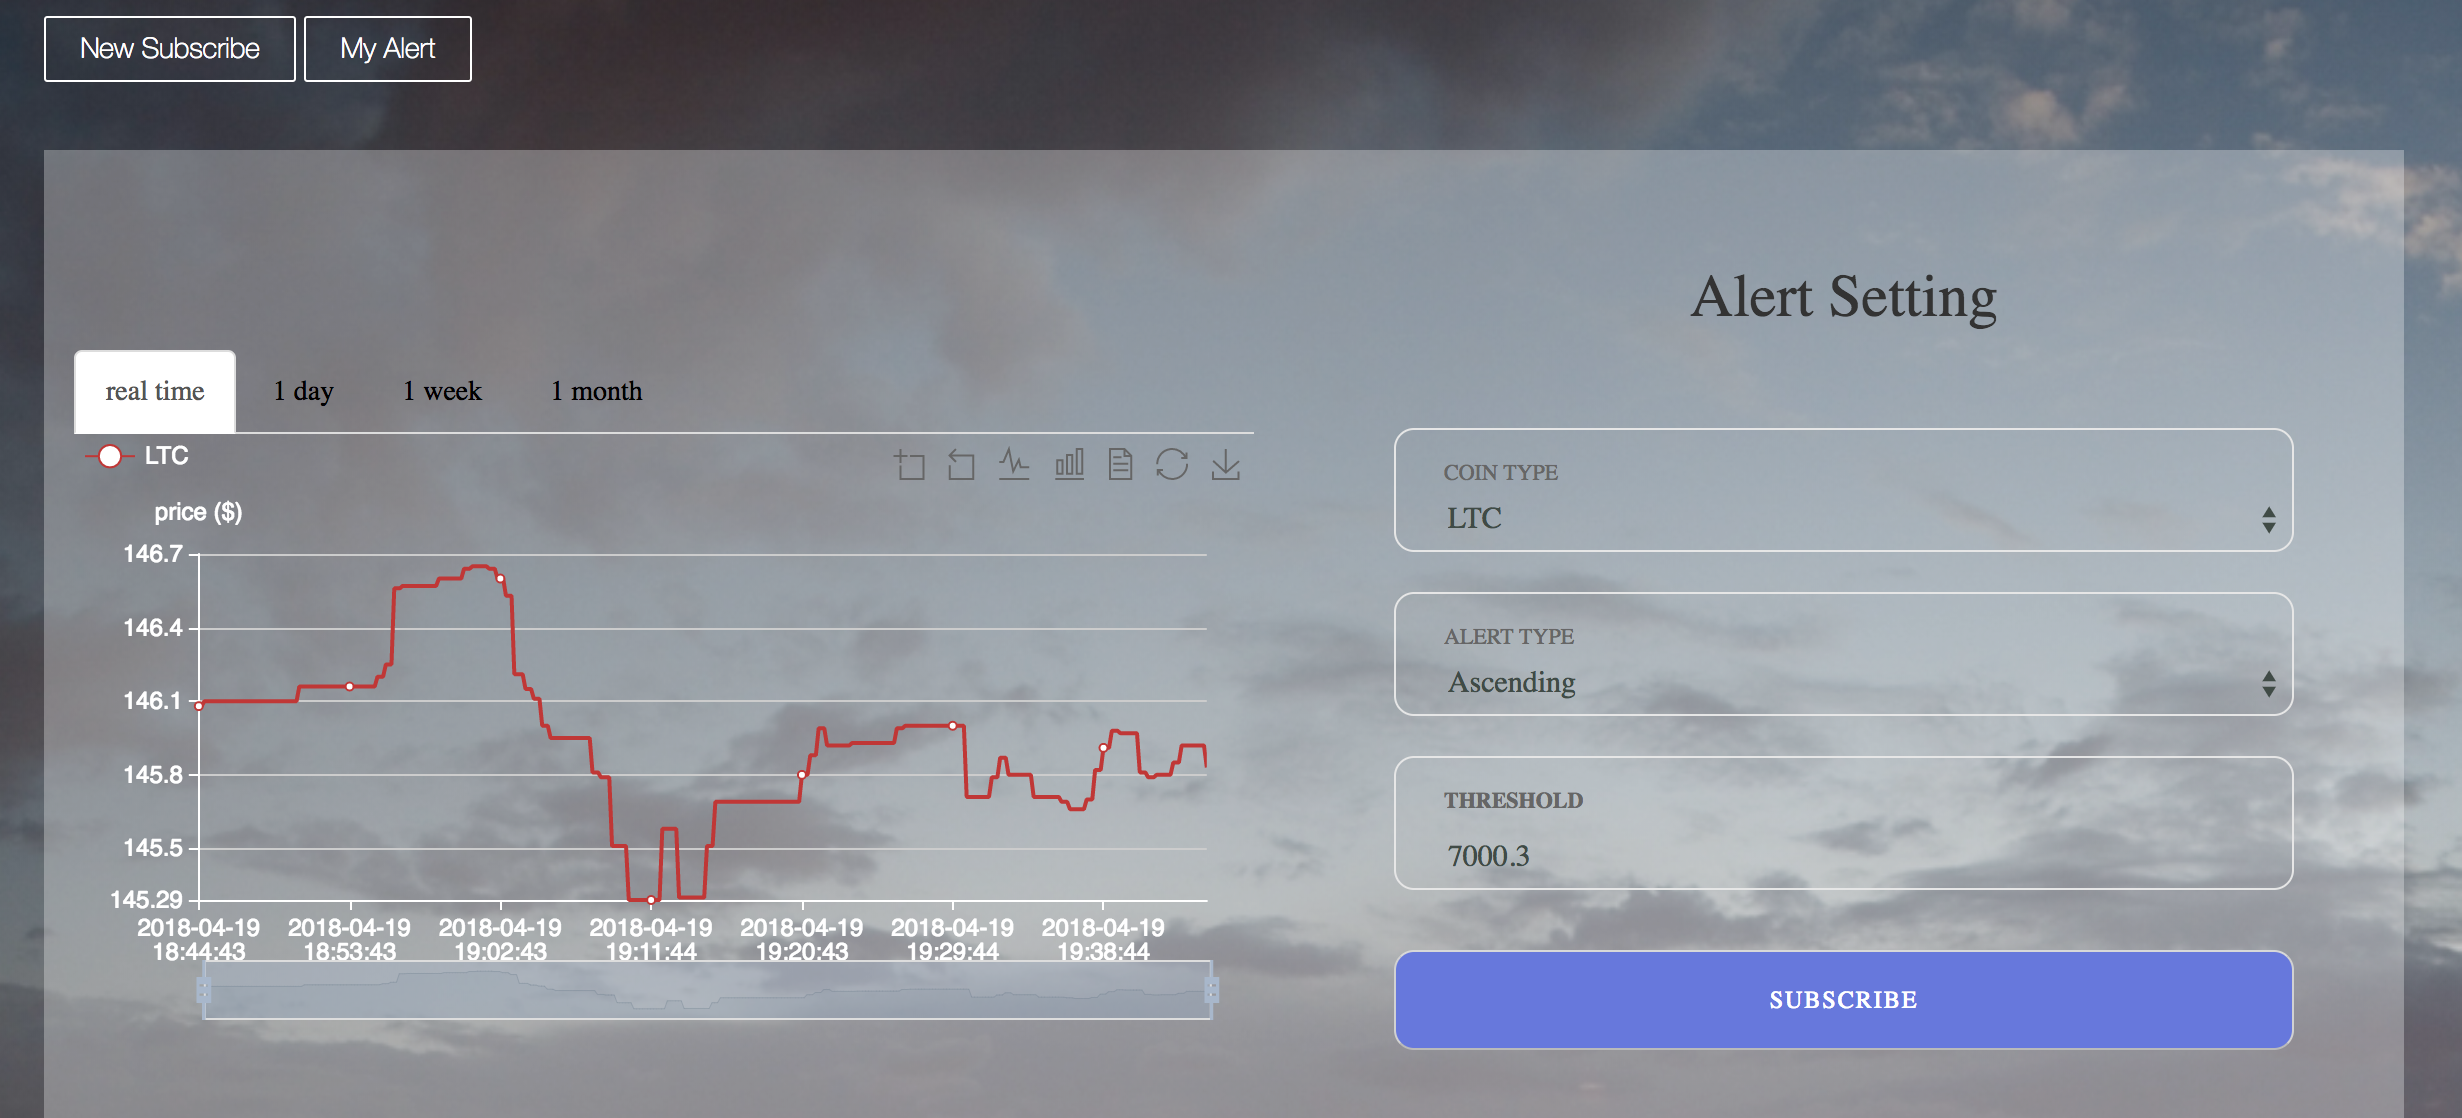
\includegraphics[height=1.5in, width=3.5in]{alert.png}
\caption{\texttt{Alert Page}}
\end{figure}


To check all the alerts that the user have, the user can click my alert on alert page,
the user can delete the alert by clicking the trash icon.

\begin{figure}[!htb]
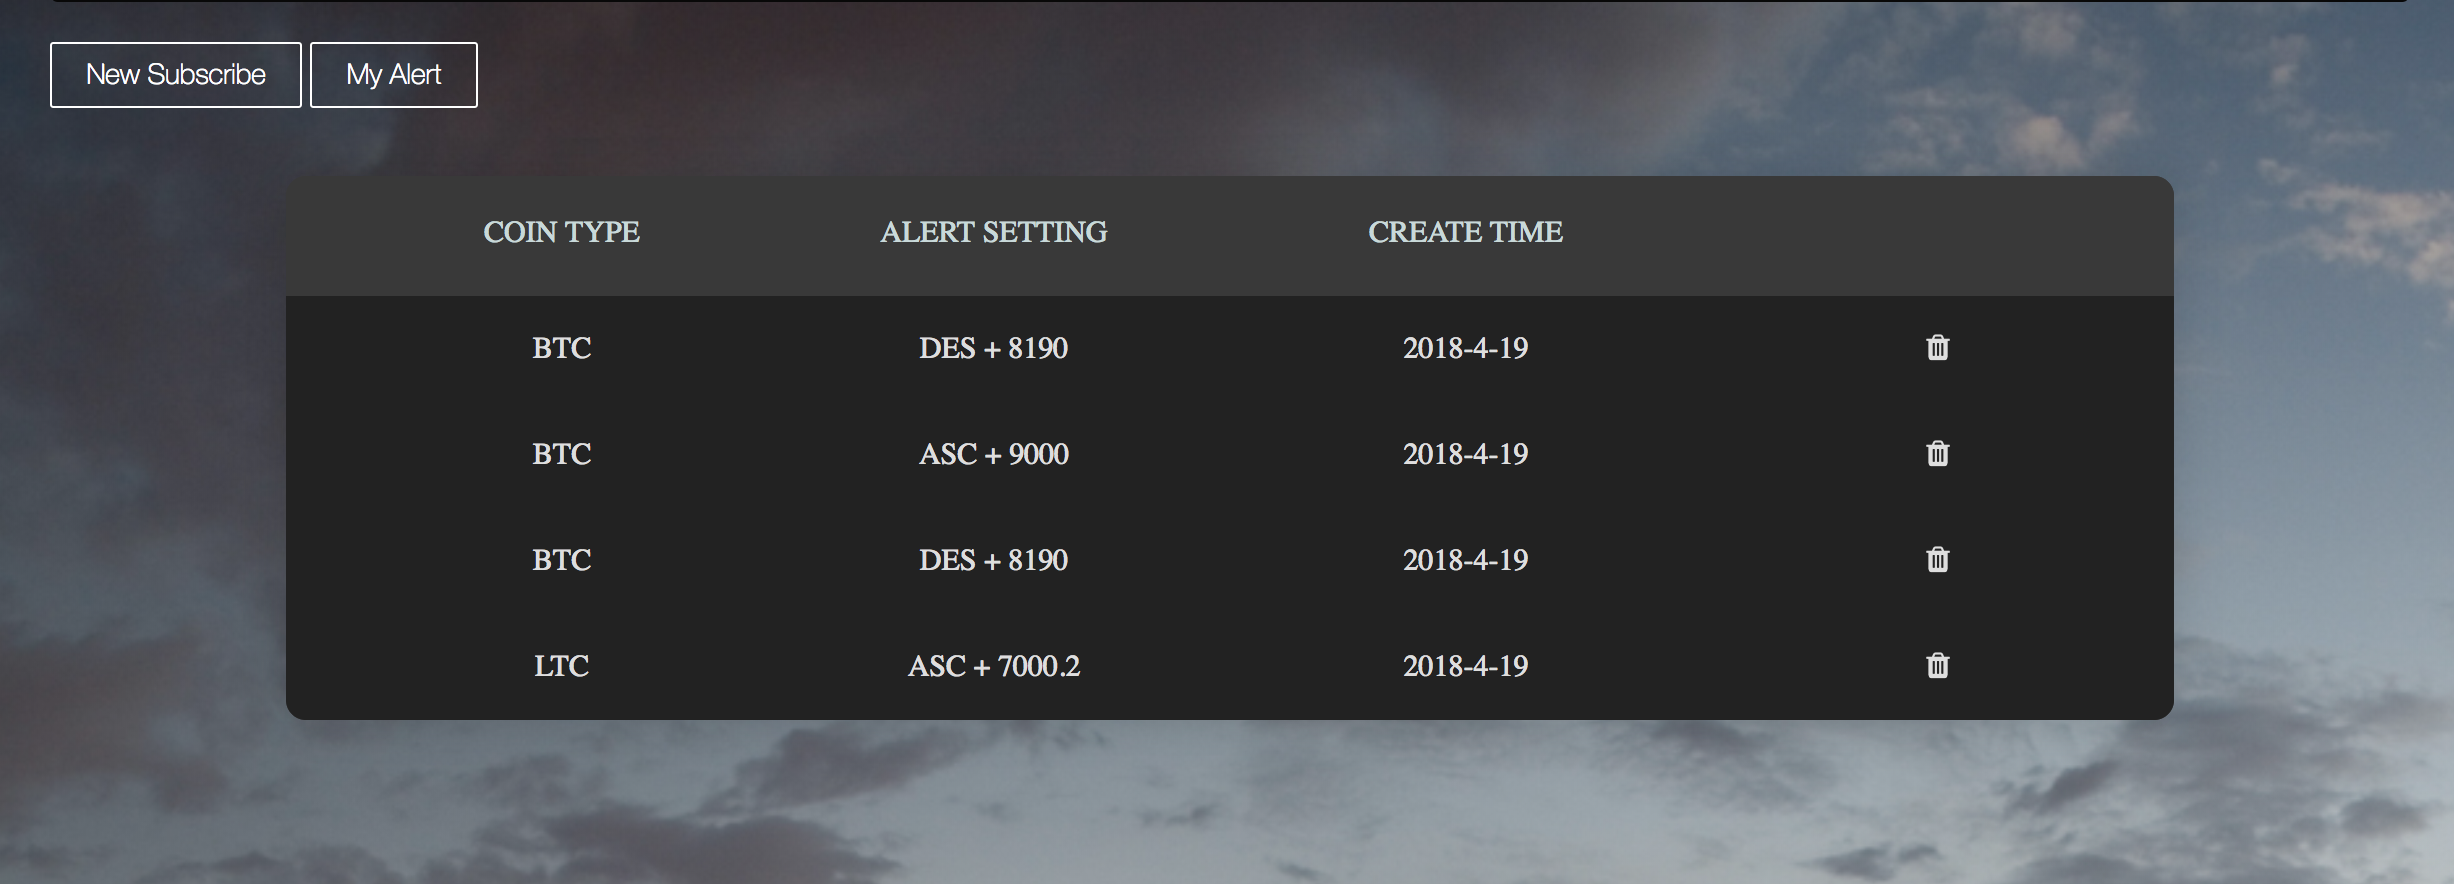
\includegraphics[height=1.5in, width=3.5in]{myalert.png}
\caption{\texttt{My Alert Page}}
\end{figure}

\subsection{Message Page}
The user can check all the messages the server sent him/her by clicking my alert on alert
page. Also the message page provide the function to filter all the message, including filter
the messages by coin type, filter the messages by alert type.

\begin{figure}[!htb]
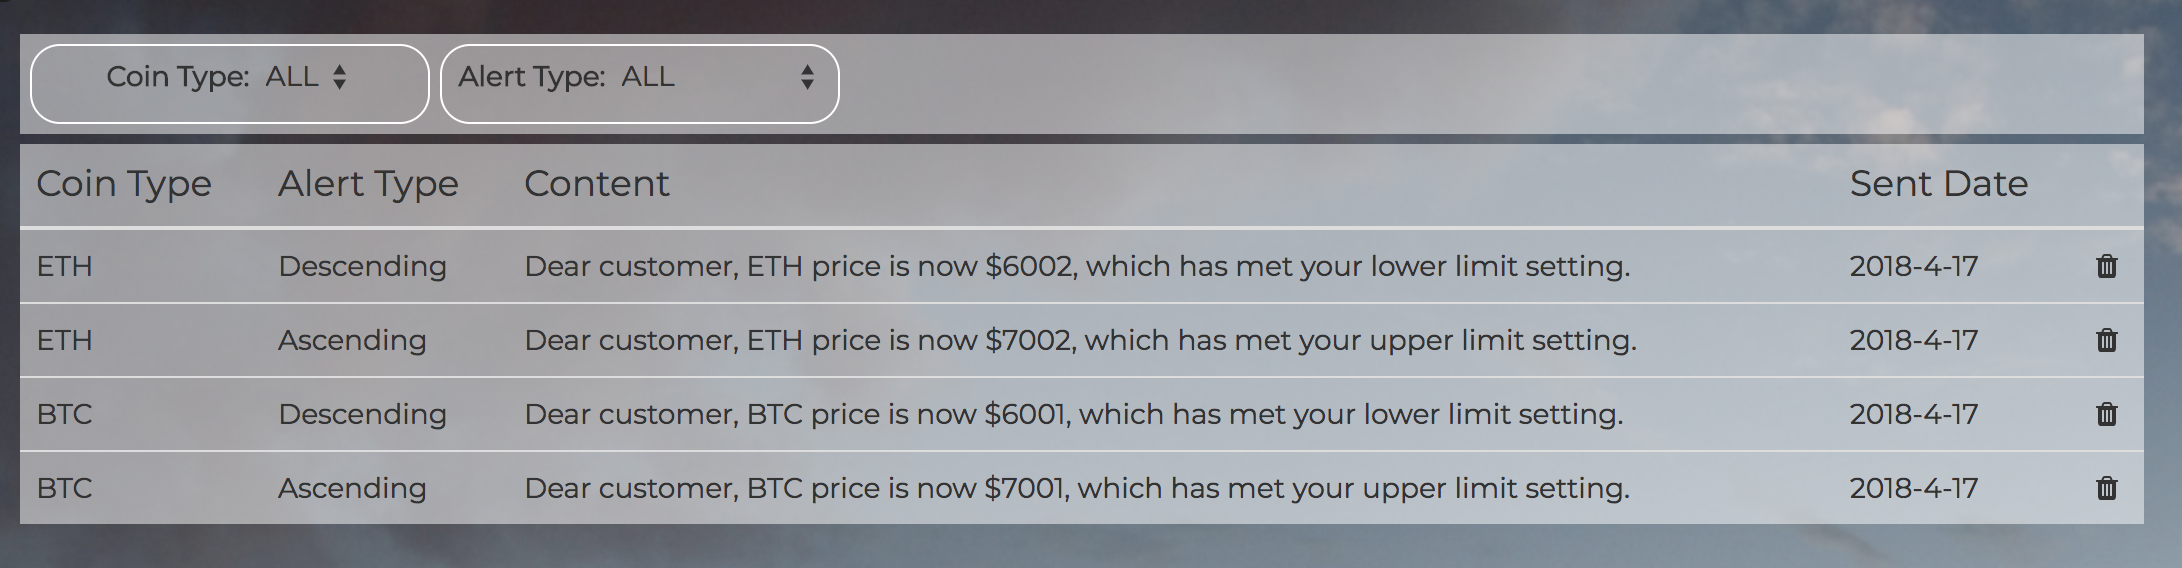
\includegraphics[height=1.0in, width=3.5in]{message.png}
\caption{\texttt{Message Page}}
\end{figure}





\section{Server-side state}
\subsection{Database Entities}
We store some entities permanently in postgres db at server-side. 
These entities include person, alert-setting and messages. 
A person has an id, name, email, hashed\_password, provider 
(google or github) and a token from provider. An alert-setting 
has an id, threshold, coin\_type (BTC, ETH or LTC), alert\_type 
(ascending or discending) and a person\_id as foreign key. 
A message has an id, content, coin\_type and alert\_type used 
for filtering at front-end. Browser can access and update/delete 
these entities through corresponding APIs and controllers using 
ajax call, and ajax callback would dispatch the front-end store 
and reflect changes.
\subsection{Agent State}
Apart from those in-database entities, real-time prices of 
cryptocurrencies are stored in Phoenix Agent and pushed to 
browser through web-socket by Phoenix Channel. The real-time 
price data is fetched from coinbase API through our server-side 
Nodejs client and supplied to Phoenix Agent through web-socket, 
too. In the Phoenix Agent, the state of real-time prices has 
a structure like this: 
\begin{center} 
\%{"BTC" => [], "ETH" => [], "LTC" => [], "time" => []}, 
\end{center}
where a series of prices in last 5000 seconds 
with 10 seconds as interval for each cryptocurrency is stored, 
also the corresponding timestamps are stored. The series of prices 
and timestamps have a maximum length of 500, which is maintained 
by the Nodejs client. These real-time prices are used to support 
the front-end echarts for users to observe a real-time price 
change in 5000 seconds. 
\subsection{Structures in Store}
We maintained a store to create and manage a set of data structures, 
utilizing Redux to combine these structures into a completed state 
for components to render. Data structures in store include: "users" 
that contains all users in our application, "token" contains the 
token of current user, "login" contains login information, "signup" 
contains register information, "alerts" contains all the alerts set 
by current user, "messages" contains all the emails that have been 
sent to current user, "current\_coin\_type" represents which type of 
coin user is viewing, "prices" contains the real time prices for 
coins, "historical\_prices" contains historical prices for coins.



\section{Related API}
\subsection{Coinbase}
We used Coinbase API to get real time prices for coins. Real 
time price provides important information for users to keep 
track of the newest status of interested coins. User behaviors 
like purchase and sell are closely related to real time price. 
Besides, real time price is the foundation of other functionalities 
of our application, like sending messages when the price reached 
certain threshold configured by users. Coinbase provides simple 
API to get real time price of different coin types. On the server 
side, we got real time price every five seconds, then pushed price 
into browser-side state through web socket.


\subsection{Crypto Compare}
We used CryptoCompare API to get historical prices for coins. 
Historical price data can provide users a straightforward sense 
of the trending and potential of coins, which is necessary for 
users to make trading decision. And CryptoCompare provides free 
and concise API to get historical price data. It parameters to 
set the time period to aggregate the data over (for daily it's 
days, for hourly it's hours) and the number of data points to 
return. We used CryptoCompare to get the past 24 hours, one week, 
one month, six months and one year's history prices for coins, 
saving these prices into state and rending them into charts and tables.
\subsection{Crypto Coins News API}
We use crypto coins news api, which provides breaking cryptocurrency
news - focusing on Bitcoin, Ethereum, ICOs, blockchain technology,
and smart contracts. We can fetch all the news in JSON format by
using AJAX's GET method. To display the news, we use title, description,
and URL of that JSON data. Every time the user enter our page, the 
page will display the top 5 crypto news. In this way, the user 
can know the latest news of cryptocurrency.
\subsection{OAuth API(Google and Github)}



\section{Complex part of application}
\subsection{Real Time Prices Monitoring at Server Side}
A complex part of our app is finding a way to monitor real-time 
prices for cryptocurrencies at server-side. This is necessary 
because our app needs to: 
\begin{itemize}
\item 1. reflect real-time price change 
through e-charts, 
\item 2. send user alert emails based on the 
real-time price change. 
\end{itemize}
Actually, it is the second point 
makes it necessary to monitor real-time prices in server 
instead of in browser. However, we used coinbase as external 
API to get real-time price data, but it doesn't supply a 
Phoenix/Elixir SDK, so we need to find a work-around. 

Our solution is building a server-side Nodejs client, which 
could work with a corresponding SDK from coinbase and connect 
with Phoenix server through websocket. In the Nodejs client, 
we used a recursive setTimeout function to fetch real-time 
price data every 10 seconds, and we used Phoenix Channel to 
push the data to Phoenix server through websocket. Since the 
real-time browser data is also supplied through websocket, 
it's convenient to let Nodejs client and browsers join at 
the same channel, so every price update in Nodejs client 
could reflect in browsers through this channel. Since the 
Nodejs client is deployed on server and is the only data 
source to update price data in channel, thus the monitoring 
of real-time price data on server is implemented.

\subsection{Display Data via Chart}
To give users a clear and straightforward presentation of 
coin prices, in “PriceChartComponent”, we utilized Echarts 
to draw the chart for real time prices and historical prices 
of selected coin. While implementing this component, first we 
need to distinguish real time price and historical price, 
because real time price is pushed by server through socket 
and history price is returned by API request. To achieve that, 
we maintained a variable to indicate whether user wanted to 
view real time price chart or historical chart, detecting 
whether the variable need to be toggled after each user 
selection. Besides, since we provided three different coin 
types, the chart should have ability to show price of different 
coin types in a single component. To achieve that, we maintained 
a “current\_coin\_type” variable in state to indicate current 
coin type being selected. Based on the value of this variable, 
chart will show corresponding prices for specific coin type. 
Also, we need to adjust the apperance of the chart (like 
font, color, axis) to keep consistency with the overall page style.


\section{Challenges and Solutions}
\subsection{Authentication with Social Media Account}
A challenge we faced was implementing login with Github/Google 
in our SPA. The auth controller in Phoenix works well with 
html.eex templates by putting call-back user information in 
session. However our app is a SPA that maintains a browser-side 
state as store, which is not easy to get user information from 
session. Besides, our app supports signup/signin with out website
account instead of Github or Google, it is uneasy to integrate 
three type of users together and let them behave equivalenty.

Our solution is giving every user a server-generated token with 
Token.sign and use this token to uniform users from different 
login providers. For our own users, the token is generated at 
TokenController as soon as they successfully login, and is sent 
back to browser through ajax callback. As for user login by 
providers, their user\_id is first fetched at PageController 
from session, and the token is generated at PageController and 
sent to browsers through window variable. Furthermore, the user 
information in session will be removed at PageController to avoid 
confusion in the future. Our front-end app component will mount 
to detect token from cookies and token from window variable to 
update the login status.

\subsection{Alert Email Distribution}




\begin{comment}

\begin{acks}
\end{acks}

\subsection{Type Changes and {\itshape Special} Characters}

We have already seen several typeface changes in this sample.  You can
indicate italicized words or phrases in your text with the command
\texttt{{\char'134}textit}; emboldening with the command
\texttt{{\char'134}textbf} and typewriter-style (for instance, for
computer code) with \texttt{{\char'134}texttt}.  But remember, you do
not have to indicate typestyle changes when such changes are part of
the \textit{structural} elements of your article; for instance, the
heading of this subsection will be in a sans serif\footnote{Another
  footnote here.  Let's make this a rather long one to see how it
  looks.} typeface, but that is handled by the document class file.
Take care with the use of\footnote{Another footnote.}  the
curly braces in typeface changes; they mark the beginning and end of
the text that is to be in the different typeface.

You can use whatever symbols, accented characters, or non-English
characters you need anywhere in your document; you can find a complete
list of what is available in the \textit{\LaTeX\ User's Guide}
\cite{Lamport:LaTeX}.

\subsection{Math Equations}
You may want to display math equations in three distinct styles:
inline, numbered or non-numbered display.  Each of
the three are discussed in the next sections.

\subsubsection{Inline (In-text) Equations}
A formula that appears in the running text is called an
inline or in-text formula.  It is produced by the
\textbf{math} environment, which can be
invoked with the usual \texttt{{\char'134}begin\,\ldots{\char'134}end}
construction or with the short form \texttt{\$\,\ldots\$}. You
can use any of the symbols and structures,
from $\alpha$ to $\omega$, available in
\LaTeX~\cite{Lamport:LaTeX}; this section will simply show a
few examples of in-text equations in context. Notice how
this equation:
\begin{math}
  \lim_{n\rightarrow \infty}x=0
\end{math},
set here in in-line math style, looks slightly different when
set in display style.  (See next section).

\subsubsection{Display Equations}
A numbered display equation---one set off by vertical space from the
text and centered horizontally---is produced by the \textbf{equation}
environment. An unnumbered display equation is produced by the
\textbf{displaymath} environment.

Again, in either environment, you can use any of the symbols
and structures available in \LaTeX\@; this section will just
give a couple of examples of display equations in context.
First, consider the equation, shown as an inline equation above:
\begin{equation}
  \lim_{n\rightarrow \infty}x=0
\end{equation}
Notice how it is formatted somewhat differently in
the \textbf{displaymath}
environment.  Now, we'll enter an unnumbered equation:
\begin{displaymath}
  \sum_{i=0}^{\infty} x + 1
\end{displaymath}
and follow it with another numbered equation:
\begin{equation}
  \sum_{i=0}^{\infty}x_i=\int_{0}^{\pi+2} f
\end{equation}
just to demonstrate \LaTeX's able handling of numbering.

\subsection{Citations}
Citations to articles~\cite{bowman:reasoning,
clark:pct, braams:babel, herlihy:methodology},
conference proceedings~\cite{clark:pct} or maybe
books \cite{Lamport:LaTeX, salas:calculus} listed
in the Bibliography section of your
article will occur throughout the text of your article.
You should use BibTeX to automatically produce this bibliography;
you simply need to insert one of several citation commands with
a key of the item cited in the proper location in
the \texttt{.tex} file~\cite{Lamport:LaTeX}.
The key is a short reference you invent to uniquely
identify each work; in this sample document, the key is
the first author's surname and a
word from the title.  This identifying key is included
with each item in the \texttt{.bib} file for your article.

The details of the construction of the \texttt{.bib} file
are beyond the scope of this sample document, but more
information can be found in the \textit{Author's Guide},
and exhaustive details in the \textit{\LaTeX\ User's
Guide} by Lamport~\shortcite{Lamport:LaTeX}.

This article shows only the plainest form
of the citation command, using \texttt{{\char'134}cite}.

Some examples.  A paginated journal article \cite{Abril07}, an enumerated
journal article \cite{Cohen07}, a reference to an entire issue \cite{JCohen96},
a monograph (whole book) \cite{Kosiur01}, a monograph/whole book in a series (see 2a in spec. document)
\cite{Harel79}, a divisible-book such as an anthology or compilation \cite{Editor00}
followed by the same example, however we only output the series if the volume number is given
\cite{Editor00a} (so Editor00a's series should NOT be present since it has no vol. no.),
a chapter in a divisible book \cite{Spector90}, a chapter in a divisible book
in a series \cite{Douglass98}, a multi-volume work as book \cite{Knuth97},
an article in a proceedings (of a conference, symposium, workshop for example)
(paginated proceedings article) \cite{Andler79}, a proceedings article
with all possible elements \cite{Smith10}, an example of an enumerated
proceedings article \cite{VanGundy07},
an informally published work \cite{Harel78}, a doctoral dissertation \cite{Clarkson85},
a master's thesis: \cite{anisi03}, an online document / world wide web
resource \cite{Thrun02d}, a video game (Case 1) \cite{Wikipedia} and (Case 2) \cite{CS188}



\subsection{Tables}
Because tables cannot be split across pages, the best
placement for them is typically the top of the page
nearest their initial cite.  To
ensure this proper ``floating'' placement of tables, use the
environment \textbf{table} to enclose the table's contents and
the table caption.  The contents of the table itself must go
in the \textbf{tabular} environment, to
be aligned properly in rows and columns, with the desired
horizontal and vertical rules.  Again, detailed instructions
on \textbf{tabular} material
are found in the \textit{\LaTeX\ User's Guide}.

Immediately following this sentence is the point at which
Table~\ref{tab:freq} is included in the input file; compare the
placement of the table here with the table in the printed
output of this document.

\begin{table}
  \caption{Frequency of Special Characters}
  \label{tab:freq}
  \begin{tabular}{ccl}
    \toprule
    Non-English or Math&Frequency&Comments\\
    \midrule
    \O & 1 in 1,000& For Swedish names\\
    $\pi$ & 1 in 5& Common in math\\
    \$ & 4 in 5 & Used in business\\
    $\Psi^2_1$ & 1 in 40,000& Unexplained usage\\
  \bottomrule
\end{tabular}
\end{table}

To set a wider table, which takes up the whole width of the page's
live area, use the environment \textbf{table*} to enclose the table's
contents and the table caption.  As with a single-column table, this
wide table will ``float'' to a location deemed more desirable.
Immediately following this sentence is the point at which
Table~\ref{tab:commands} is included in the input file; again, it is
instructive to compare the placement of the table here with the table
in the printed output of this document.


\begin{table*}
  \caption{Some Typical Commands}
  \label{tab:commands}
  \begin{tabular}{ccl}
    \toprule
    Command &A Number & Comments\\
    \midrule
    \texttt{{\char'134}author} & 100& Author \\
    \texttt{{\char'134}table}& 300 & For tables\\
    \texttt{{\char'134}table*}& 400& For wider tables\\
    \bottomrule
  \end{tabular}
\end{table*}
% end the environment with {table*}, NOTE not {table}!



\subsection{Figures}

Like tables, figures cannot be split across pages; the best placement
for them is typically the top or the bottom of the page nearest their
initial cite.  To ensure this proper ``floating'' placement of
figures, use the environment \textbf{figure} to enclose the figure and
its caption.

This sample document contains examples of \texttt{.eps} files to be
displayable with \LaTeX.  If you work with pdf\LaTeX, use files in the
\texttt{.pdf} format.  Note that most modern \TeX\ systems will convert
\texttt{.eps} to \texttt{.pdf} for you on the fly.  More details on
each of these are found in the \textit{Author's Guide}.

\begin{figure}
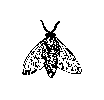
\includegraphics{fly}
\caption{A sample black and white graphic.}
\end{figure}

\begin{figure}
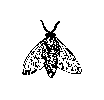
\includegraphics[height=1in, width=1in]{fly}
\caption{A sample black and white graphic
that has been resized with the \texttt{includegraphics} command.}
\end{figure}




\begin{figure*}
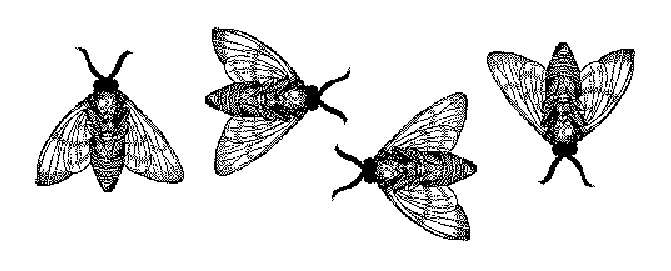
\includegraphics{flies}
\caption{A sample black and white graphic
that needs to span two columns of text.}
\end{figure*}


\begin{figure}
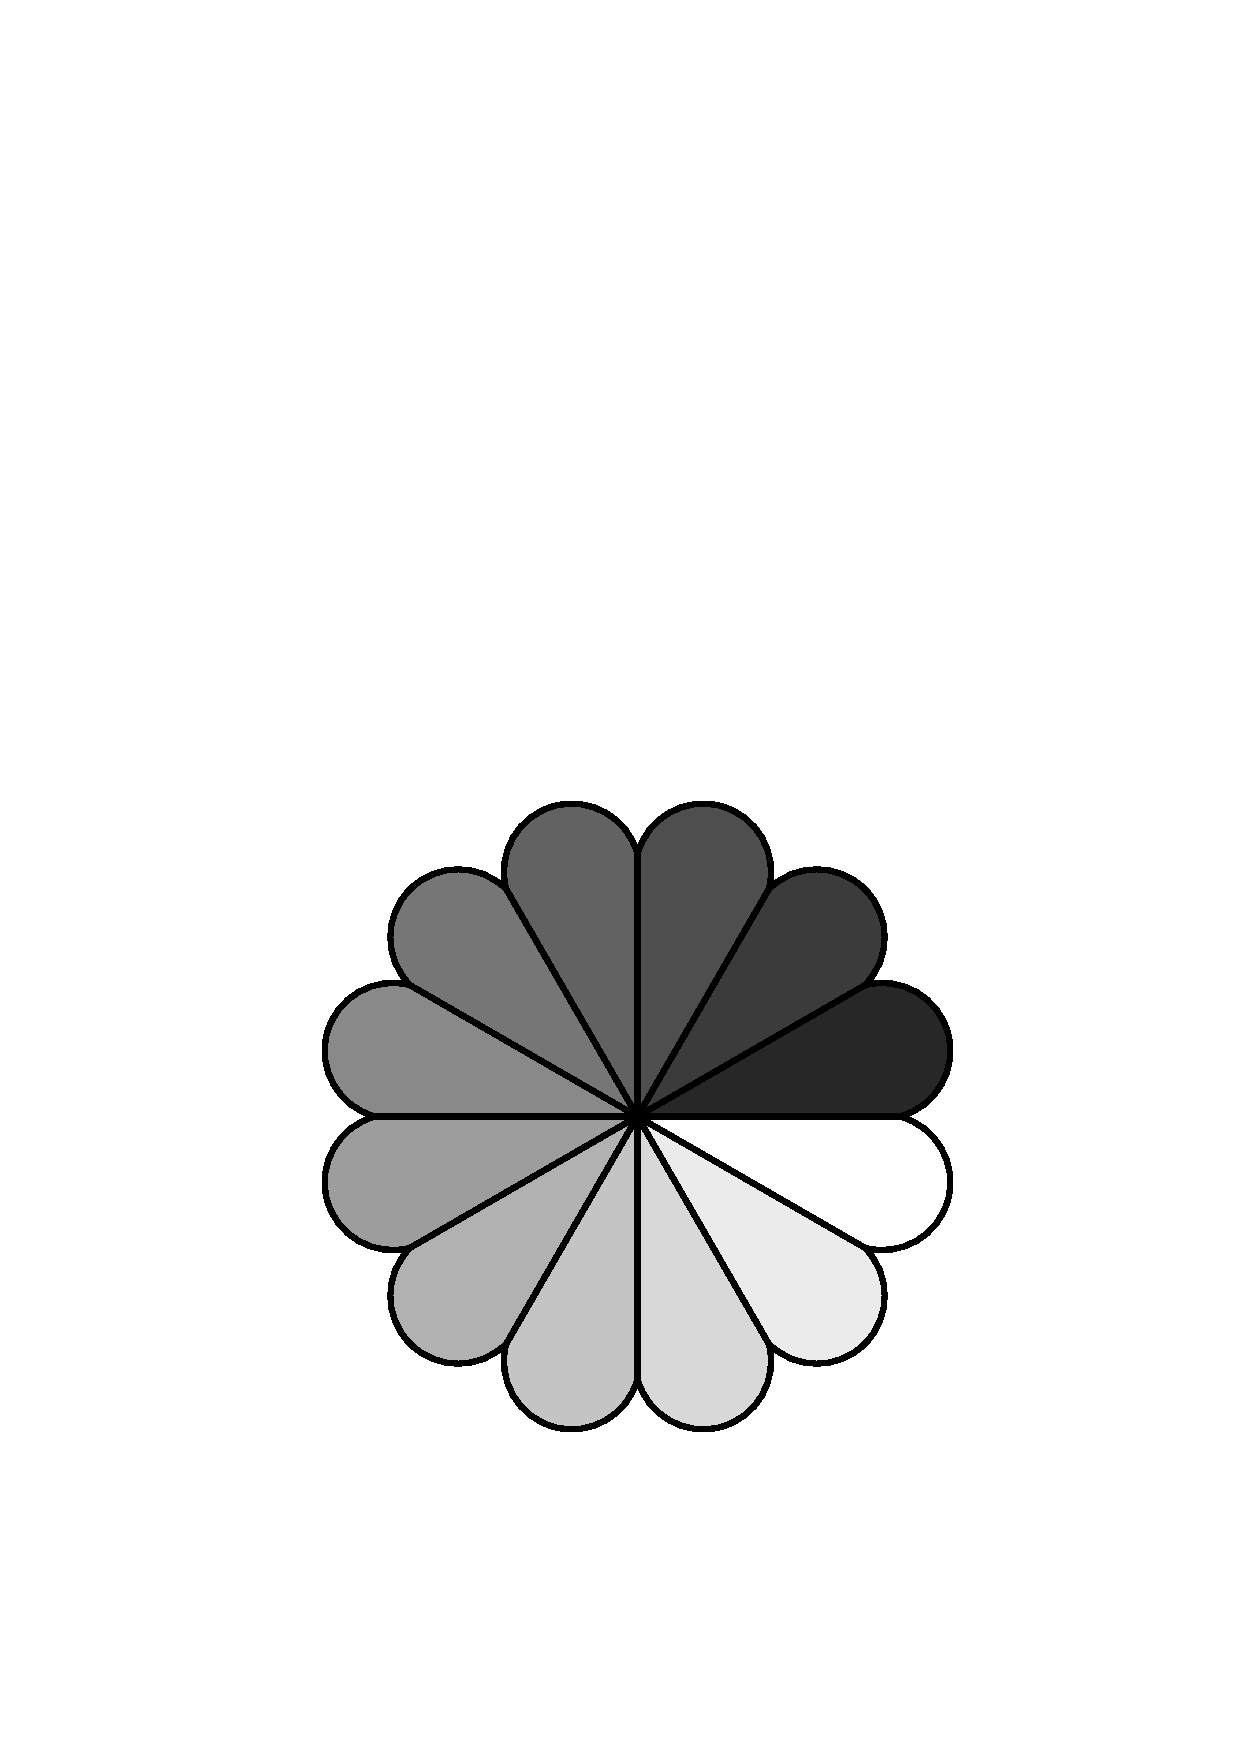
\includegraphics[height=1in, width=1in]{rosette}
\caption{A sample black and white graphic that has
been resized with the \texttt{includegraphics} command.}
\end{figure}


%\end{document}  % This is where a 'short' article might terminate



\appendix
%Appendix A
\section{Headings in Appendices}
The rules about hierarchical headings discussed above for
the body of the article are different in the appendices.
In the \textbf{appendix} environment, the command
\textbf{section} is used to
indicate the start of each Appendix, with alphabetic order
designation (i.e., the first is A, the second B, etc.) and
a title (if you include one).  So, if you need
hierarchical structure
\textit{within} an Appendix, start with \textbf{subsection} as the
highest level. Here is an outline of the body of this
document in Appendix-appropriate form:
\subsection{Introduction}
\subsection{The Body of the Paper}
\subsubsection{Type Changes and  Special Characters}
\subsubsection{Math Equations}
\paragraph{Inline (In-text) Equations}
\paragraph{Display Equations}
\subsubsection{Citations}
\subsubsection{Tables}
\subsubsection{Figures}
\subsubsection{Theorem-like Constructs}
\subsubsection*{A Caveat for the \TeX\ Expert}
\subsection{Conclusions}
\subsection{References}
Generated by bibtex from your \texttt{.bib} file.  Run latex,
then bibtex, then latex twice (to resolve references)
to create the \texttt{.bbl} file.  Insert that \texttt{.bbl}
file into the \texttt{.tex} source file and comment out
the command \texttt{{\char'134}thebibliography}.
% This next section command marks the start of
% Appendix B, and does not continue the present hierarchy
\section{More Help for the Hardy}

Of course, reading the source code is always useful.  The file
\path{acmart.pdf} contains both the user guide and the commented
code.
\end{comment}




%%%%%%%%%%%%%%%%%%%%%%%%%%%%%%%%%%%%%%%%%%%%%%%%%%%%%%%%%%%%%%%%%%%%%%%%%%%%%%%%%%%%%%%%%%%%%%%%%%%%%%%%%
%% bibliography: see CFP for number of permitted pages

%\bibliographystyle{ACM-Reference-Format}  % do not change this line!
\bibliography{sample-bibliography}  % put name of your .bib file here

\end{document}
